\chapter{Graph Databases}
    First, we introduce a popular data model employed by many current graph databases~\autocite{GitHubneo4j, ArangoDB, AmazonNeptune, RedisGraph}.
    Then we look at an implementation of this model in a native graph database called Neo4J is described. 
    The latter also serves as a role model for implementing the in-memory database used in the evaluation part.
                
    \section{Architecture}
        Graph databases do not differ in many architectural aspects from relational and other databases. A sketch of the software architecture of database management systems is laid out in Section~\ref{db-arch}. 
        The most significant difference is how data is stored on the one hand side and how the queries are evaluated on the other hand side.
        As mentioned, we focus on the former issue.
        
        Relational databases store data in tables.
        The links considered in this category of DBMS are primarily used to stitch together the fields of a record stored in different tables into one row again after the split to satisfy a particular normal form.
        One may also store tables where one table stores nodes and the other table's fields are node IDs to represent relationships.

        However, to traverse the graph, one either has to do many rather expensive lookups or store auxiliary structures to speed up the lookup process.
        In particular, when using B-trees as index structure, each lookup takes $\mathcal{O}(\log(n))$ steps for clustered indices to locate a specific edge. However, as all edges are attached to two nodes, it is only possible to build an unclustered index over edges either grouped by incoming or outgoing neighborhood. The undirected neighborhood permits no such sorting and retrieval as it is unclear to which node an edge is to be sorted.
        Alternatively, one could store an additional table that holds incidence lists such that the lookup of outgoing or incoming edges is only $\mathcal{O}(\log(n))$ which would speed up breadth-first traversals, but duplicate data.
        Still, one has to compute joins to continue the traversal in the scope of depth-first searches.
        Another way to speed things up is to use a hash-based index, but this also has an unavoidable overhead aside from the joins and the question of which hash function and which attributes to use arises.
        
        In contrast to relational databases, native graph databases use structures specialized for these kinds of queries.
            
    \section{The Property Graph Model}\label{prop-graph-model}
        The property graph model is a widely adopted data model to represent graphs in databases.
        It can represent the structure of directed or undirected, weighted or unweighted, and typed graphs having additional properties.

        A \textbf{Property Graph} is a 9-Tuple $G = (V, E, \lambda, P, T, L, f_P, f_T, f_L)$ with 
        \begin{itemize}
            \item $V$ the set of vertices.
            \item $E$ the set of edges.
            \item $\lambda: (V \times V) \rightarrow E$ a binary relation assigning a pair of nodes to an edge.
            \item $P$ a set of key-value pairs called properties.
            \item $T$ a set of strings used as relationship types.
            \item $L$ a set of strings used as labels.
            \item $f_P: V \cup E \rightarrow 2^P$ a binary relation that assigns a set of properties to a node or relationship.
            \item $f_T: E \rightarrow T$ a binary relation that assigns a type to a relationship.
            \item  $f_L: V \rightarrow 2^L$ a binary relation that assigns a node a set of labels.
        \end{itemize} 
        \smallskip
        The property graph model reflects a directed, node-labeled and relationship-typed multigraph $G$, where each node and relationship can hold a set of properties~\cite{angles2018property, rodriguez2012graph, Rodriguez2010ConstructionsFD}.
        In a graph, the edges are usually defined as $E \subseteq (V \times V)$, but in the property graph model, edges have sets of properties and a type, making them records independently. 
        An illustration of this model is shown in Figure~\ref{propertygraph}.
        
        \begin{figure}[htp]
            \begin{center}
                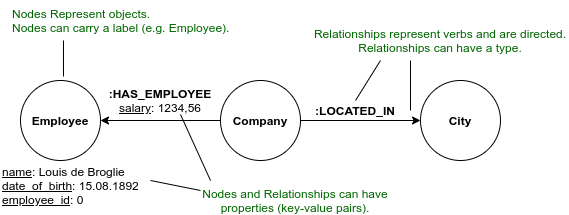
\includegraphics[keepaspectratio,width=\textwidth]{img/04-databases/property_graph_elements.png}
            \end{center}
            \caption{A schematic visualization of the property graph model.} 
            \label{propertygraph}
        \end{figure}

        
        Neo4j is a graph database employing the property graph model~\cite{robinson2015graph}.
        The logical operators of this model are described in~\autocite{Holsch2016Algeb}. 
        The \textit{get\_nodes}-operator returns all nodes of the graph.
        No matter how the nodes are stored, the whole file (portion) needs to be scanned.
        Furthermore, the \textit{expand}-operator returns the incident edges of a node depending on the direction.
        Expand only considers a part of all edges, so it does not do full scans but somewhat smaller reads.
        Finally, the \textit{filter}-operand selects specific nodes or relationships based on properties, labels or, relationship type.
        
        In the next Section~\ref{n4j} we are going to discuss how Neo4J implements the property graph model, with our focus on the structure of the graph and the low-level storage scheme.

\section{Neo4J}\label{n4j}
    Neo4J is a native graph database using the property graph model.
    The source code of the community edition is available at GitHub~\autocite{GitHubneo4j}.
    We look at some implementation details of the storage and buffer manager and the record structure.
    We will not take properties, relationship types, labels, and concepts related to those into account.
    
    \subsection{High-level Architecture}
        \begin{figure}[htp]
            \begin{center}
                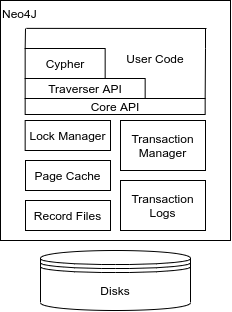
\includegraphics[keepaspectratio,width=0.25\textwidth]{img/04-databases/N4J_HLA_Emil.png}
            \end{center}
            \caption{The high level architecture of Neo4J~\autocite{robinson2015graph}.} 
            \label{N4J_HLA_Emil}
        \end{figure}
        
        To get an overview of the architecture, let us consider Figure~\ref{N4J_HLA_Emil}.
        This description was outlined by the co-founder of Neo4J Emil Effrem, the chief science officer Jim Webber and Ian Robinson, a former engineer at Neo4J, in their book on graph databases~\autocite{robinson2015graph}.
        Here we can see that the architectural schema outlined in Section~\ref{db-arch} and especially Section~\ref{dbms_arch} was not entirely applied.
        
        Still, the components are very similar.
        The ''Page Cache`` is equivalent to the buffer manager, the record files are what is managed by the disk space manager, mechanisms to deal with free slots~\autocite{neo4jidgenerator} and (de-)allocations~\autocite{neo4jio} are also part of the software stack, as are the record formats~\autocite{neo4jrecordstorage} and indexes, corresponding to the access layer. 
        The corresponding components are just put together in a slightly different manner. 
        
        \begin{figure}[htp]
            \begin{center}
                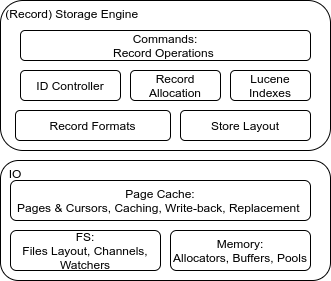
\includegraphics[keepaspectratio,width=0.33\textwidth,height=0.3\textheight]{img/04-databases/N4J_Storage.png}
            \end{center}
            \caption{A visualization of the broad storage and memory organization of Neo4J.} \label{N4J_Storage}
        \end{figure}
        
        The detailed composition is shown in Figure~\ref{N4J_Storage}.
        The IO package contains the page cache, which is the buffer manager.
        It also contains facilities to create, grow and shrink files using the \mintinline{java}{java.nio} library and wrappers around platform-dependent allocation facilities.
        Thus the (de-)allocation part of the disk space manager resides in the IO package, too.
        The record storage engine defines the record format and the file layout and means to create and maintain indices. Thus it is similar to the access layer. 
        It also handles the management of free slots --- something that the disk space manager usually does.
        To summarize: the buffer manager and the access layer correspond closely to these two packages, while the disk space manager is distributed mainly over these two packages.        

    \subsection{Record and File Structures}\label{n4j-struct}
        Neo4J uses several different record types. They can be split broadly in the following categories:
        \begin{itemize}
            \item Variable size records: Strings, Arrays
            \item Fixed size records:
            \begin{itemize}
            \item Graph structure related records: Nodes, relationships, relationship groups
            \item Properties, labels, relationship types
            \end{itemize}
        \end{itemize}
        
        Each record type is stored in an own file per database in the database management system.
        An additional system database keeps track of the existence and metadata of the other ones storing user data.
        This is visualized in Figure~\ref{n4j-disk}.
        \begin{figure}[htp]
            \begin{center}
                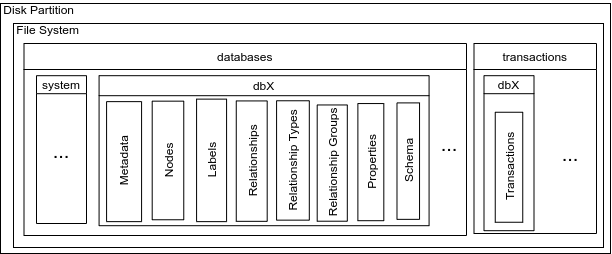
\includegraphics[keepaspectratio,height=0.4\textheight,width=0.7\textwidth]{img/04-databases/N4J_disk_view.png}
            \end{center}
            \caption{A visualization of how the files are arranged of Neo4J.}
            \label{n4j-disk}
        \end{figure}
        
        The records are ordered simply by their insertion order, i.e., the files storing the records are heap files.
        While variable-length records store strings and arrays, labels, for example, store a pointer to the actual string of the label to be fixed size and thus efficiently retrieved.
        The same is valid for relationship types and property keys and values that are strings or arrays.
        The separate storage is done to avoid duplications of strings, e.g., of each label.
        As mentioned before, we will elaborate on the elements that represent the graph structure for the sake of succinctness. 
        Only one thing is to be mentioned.
        Properties are stored as linked lists for each node and relationship.
        
    \subsubsection*{Node Records}
        \begin{figure}[htp]
            \begin{center}
                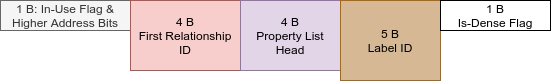
\includegraphics[keepaspectratio,height=0.4\textheight,width=0.7\textwidth]{img/04-databases/node_record.png}
            \end{center}
            \caption{A visualization of the record structure of a node record~\autocite{neo4jNodeRecordFormat}.}
            \label{node-record-format}
        \end{figure}
        The record format of nodes consists of a 15-byte structure.
        The IDs of nodes are stored implicitly as their address.
        If a node has ID 100, we know that its record starts at offset $15 \text{ Bytes} \cdot 100 = 1500$ from the beginning of the file.
        The struct of a record is outlined below.
        \begin{enumerate}
            \item Byte 1: One bit for the in-use flag. 
            The additional bits are used to compress the node struct by using the other 7 bits to store the most significant bits of the first relationship ID and the first property ID 
            \item Bytes 2 --- 5: The next 4 Bytes represent the head's relationship ID in the linked list of the considered node's relationships.
            \item Bytes 6 --- 9: Again, 4 bytes encode the head's property ID in the node's linked list of properties.
            \item Bytes 10 --- 14: This 5-byte section points to the labels of this node.
            \item Byte 15: The last byte stores if the node is dense, i.e., \ has an awful lot of relationships, such that it needs special treatment to remain efficient to traverse over.
            That is, relationships are grouped by type and direction for this node.
        \end{enumerate}
        
        To summarize: the records on disk are stored as in the enumeration above, and as shown in Figure~\ref{node-record-format}. 
        In the database, all IDs get mapped to longs, and their respective space is larger than the space representable by 35 bits --- which is perfectly fine.
        
        On-disk 4-byte integers are used to store the 32 lowest bits of the respective addresses, and the higher bits are stored in the first byte that also carries the in-use bit.
    
    \subsubsection*{Relationship Records}\label{n4j-rel}
        \begin{figure}[htp]
            \begin{center}
                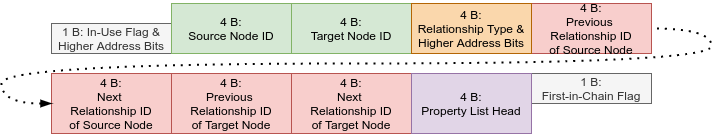
\includegraphics[keepaspectratio,height=0.9\textheight,width=0.9\textwidth]{img/04-databases/relationship_record.png}
            \end{center}
            \caption{A visualization of the record structure of a relationship in Neo4J.}
            \label{rel_record}
        \end{figure}
            
        Relationship records are stored with implicit IDs too. 
        Their fixed-size records contain 34 bytes.
        Besides an in-use flag, the source and target node IDs, and the relationship type, the record also contains two doubly-linked lists --- one for the source node's incident edges and one for the target node's incident edges.
        Next, a link to the head of the linked list of properties for this relationship is stored.
        Finally, the last byte contains a marker if this relationship is the first element in the nodes' incidence list.
        
        \begin{enumerate}
            \item Byte 1: In-use bit, source node high order bits (3 bits), first property high order bits (4 bits)
            \item Bytes 2 --- 5: source node ID 
            \item Bytes 6 --- 9: target node ID 
            \item Bytes 10 --- 13: relationship type (16 bit), target node high order bits (3 bits), relationship previous and next ID higher bits for source and target node ($4 \cdot 3 = 12$ bits), one unused bit.
            \item Bytes 14 --- 17: previous relationship ID the for source node
            \item Bytes 18 --- 21: next relationship ID for the source node
            \item Bytes 22 --- 25: previous relationship ID for the target node
            \item Bytes 26 --- 29: next relationship ID for the target node
            \item Bytes 30 --- 33: link to the first property of the relationship
            \item Bytes 34: A marker if this relation is the first element in the relationship linked list of one of the nodes stored in the byte's lowest two bits. 
            The other 6 bits are unused.
        \end{enumerate}
        
        \begin{figure}[htp]
            \begin{center}
                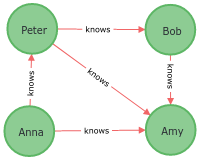
\includegraphics[keepaspectratio,height=0.4\textheight,width=0.3\textwidth]{img/04-databases/graph.png}
            \end{center}
            \caption{An example graph.}
            \label{n4j-ex-gr}
        \end{figure}
        
        The relationship structure is a crucial element of the layout and reveals the actual data type that the database is using.
        Nodes and relationships are both stored once only (i.e., nothing is duplicated).
        Without taking the fields into account, this is an unordered edge list.
        When taking the linked lists of relationships into account, it turns out that the underlying data structure is that of an incidence list, with a couple of additional properties.
        
        First, as already mentioned, the edges are not physically duplicated but only referenced. 
        The records are fixed-sized, so addressing them is done by multiplying the index by the size of an entry, meaning one does not need to store primary keys explicitly, and address translation can be done using simple multiplication. 
        Theoretically, one could align the record size to a power of two to turn the multiplication into a bit shift.
        Next, as doubly linked lists are used, the deletion of an edge is in $\mathcal{O}(1)$ if the ID is known.
This variant of deletion assumes that the doubly linked incidence lists are circular, i.e., the head's pervious element is the tail and reciprocally.
        If this were not the case, the incidence list would need to be traversed to find the last element.
        Also, the incidence list is stored in the relationships.
        Thus to traverse from one node's incidence list to another, there is no need to load the node record itself.
        It suffices to dereference the next element in the incidence list stored by the relationships and store the edge's ID that started the traversal.
        

        To conclude this example, we briefly visualize the just described storage schema. 
        The high-level graph is shown in Figure~\ref{n4j-ex-gr}.
        It contains four nodes and five edges.
        The underlying instantiated data structures are shown in Figure~\ref{n4j-ex}.
        The light red arcs represent edges; the light green circles represent nodes.
        The colored boxes on the edges and nodes represent the data structures.
        The brighter red edges represent the doubly linked incidence lists.
        Notice that the doubly linked incidence lists' heads and tails are marked by ''X`` to avoid drawing additional edges.
        The brighter green arrows represent the source and target nodes, as stored by the edges.
        \vfill
        \begin{figure}[htp]
            \begin{center}
                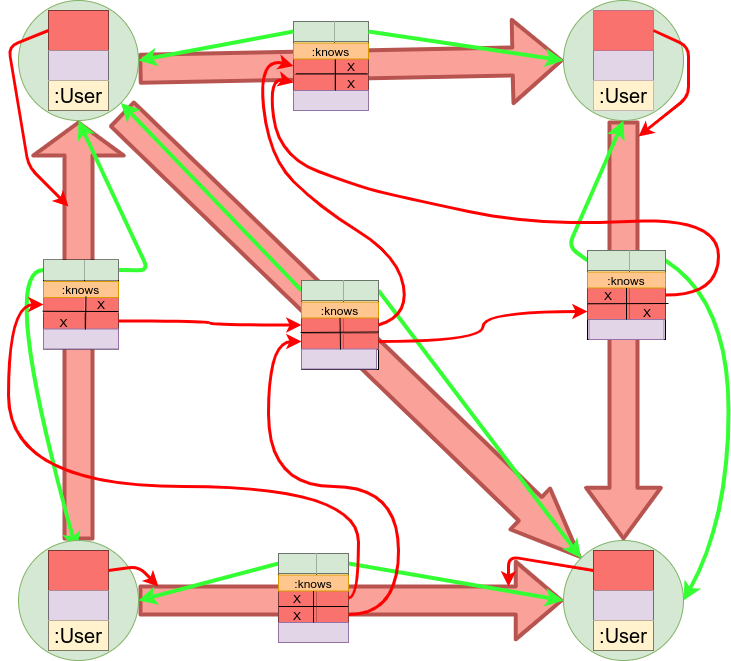
\includegraphics[keepaspectratio,height=\textheight,width=\textwidth]{img/04-databases/example_structs.png}
            \end{center}
            \caption{Visualization of the data structures, as initialized by the example graph shown in Figure~\ref{n4j-ex-gr}.}
            \label{n4j-ex}
        \end{figure}
        \vfill
